\documentclass{beamer}
% \usepackage{pgfpages}
% \pgfpagesuselayout{4 on 1}[a4paper,landscape,border shrink=5mm]
\usepackage{tikz}
\usetikzlibrary{shapes, backgrounds}
\usepackage{listings}
\usepackage[utf8,latin1]{inputenc}
\usepackage[natbibapa]{apacite}
\makeatletter \def\newblock{\beamer@newblock} \makeatother  

\beamertemplatenavigationsymbolsempty
\setbeamertemplate{itemize items}[circle]
\setbeamertemplate{section in toc}[circle]
\mode<beamer>{\setbeamercolor{math text displayed}{fg=iwmgrau}}
\setbeamercolor{block body}{bg=iwmorange!50!white}
\setbeamercolor{block title}{fg=white, bg=iwmorange}

\definecolor{iwmorange}{RGB}{255,105,0}
\definecolor{iwmgrau}{RGB}{67,79,79}
\setbeamercolor{title}{fg=iwmorange}
\setbeamercolor{frametitle}{fg=iwmorange}
\setbeamercolor{structure}{fg=iwmorange}
\setbeamercolor{normal text}{fg=iwmgrau}
\setbeamercolor{author}{fg=iwmgrau}
\setbeamercolor{date}{fg=iwmgrau}
\color{white}

\title{Regression analysis}
\author{Nora Umbach%\footnote{These slides are a modified version of slides created by \url{https://osf.io/ /}. }
}
%\institute{\includegraphics[scale=.15]{figures/ut_logo}}
\date{April 19, 2021}
%\date{Last modified: \today}

\newcommand{\vect}[1]{\mathbf{#1}}
\newcommand{\mat}[1]{\mathbf{#1}}
\newcommand{\gvect}[1]{\boldsymbol{#1}}
\newcommand{\gmat}[1]{\boldsymbol{#1}}

\lstset{language=R,%
  literate={Ü}{{\"U}}1
           {ü}{{\"u}}1,
  %backgroundcolor=\color{iwmgrau!80!white},
  basicstyle=\ttfamily\color{iwmorange},
  frame=single,
  commentstyle=\slshape\color{black},
  keywordstyle=\bfseries\color{white},
  identifierstyle=\color{white},
  stringstyle=\color{green!85!black},
  numbers=none,%left,numberstyle=\tiny,
  basewidth={.5em, .4em},
  showstringspaces=false,
  emphstyle=\color{red!50!white}}

\lstdefinestyle{plain}{language=R,
  frame=none,
  basicstyle=\ttfamily\color{iwmorange},
  commentstyle=\slshape\color{iwmgrau},
  keywordstyle=\bfseries\color{iwmgrau},
  identifierstyle=\color{iwmgrau},
  stringstyle=\color{iwmgrau},
  numbers=none,
  basewidth={.5em, .4em},
  showstringspaces=false}

\AtBeginSection[]{
  \frame{
    \tableofcontents[sectionstyle=show/hide, subsectionstyle=show/show/hide]}}

\setbeamertemplate{headline}{
 \begin{beamercolorbox}{section in head}
   \vskip5pt\insertsectionnavigationhorizontal{\paperwidth}{}{}\vskip2pt
 \end{beamercolorbox}
}

\setbeamertemplate{footline}{\vskip-2pt\hfill\insertframenumber$\;$\vskip2pt}

\begin{document}

\begin{frame}{}
\thispagestyle{empty}
\titlepage
\end{frame}

\begin{frame}{Outline}
\tableofcontents
\end{frame}


\section[Intro]{Introduction}


\begin{frame}{Problem}
\begin{columns}
\begin{column}{5cm}
For a two-dimensional scatter plot
\[
  (x_1, y_1), \ldots, (x_n, y_n)
\]
we want to fit the best possible line
\[
  \hat{y} = a + b \cdot x
\]
\end{column}
%
\begin{column}{6cm}
% Created by tikzDevice version 0.6.2-92-0ad2792 on 2012-11-14 12:23:43
% !TEX encoding = UTF-8 Unicode
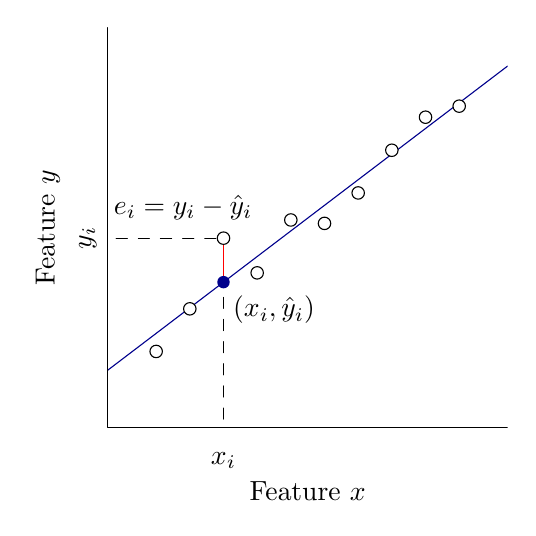
\begin{tikzpicture}[x=1pt,y=1pt]
\definecolor[named]{fillColor}{rgb}{1.00,1.00,1.00}
\path[use as bounding box,fill=fillColor,fill opacity=0.00] (0,0) rectangle (173.45,173.45);
\begin{scope}
\path[clip] (  0.00,  0.00) rectangle (173.45,173.45);
\definecolor[named]{drawColor}{rgb}{0.00,0.00,0.00}

\node[text=drawColor,anchor=base,inner sep=0pt, outer sep=0pt, scale=
  1.00] at (101.18,  2.51) {Feature $x$};

\node[text=drawColor,rotate= 90.00,anchor=base,inner sep=0pt, outer
  sep=0pt, scale=  1.00] at (  9.71,101.18) {Feature $y$};
\end{scope}
\begin{scope}
\path[clip] ( 28.91, 28.91) rectangle (173.45,173.45);
\definecolor[named]{drawColor}{rgb}{0.00,0.00,0.55}

\path[draw=drawColor,line width= 0.4pt,line join=round,line cap=round] ( 28.91, 49.66) -- (173.45,159.60);
\definecolor[named]{drawColor}{rgb}{0.00,0.00,0.00}

\path[draw=drawColor,line width= 0.4pt,dash pattern=on 4pt off 4pt ,line join=round,line cap=round] (  0.00, 97.39) --
	( 70.76, 97.39);

\path[draw=drawColor,line width= 0.4pt,dash pattern=on 4pt off 4pt ,line join=round,line cap=round] ( 70.76,  0.00) --
	( 70.76, 81.50);
\definecolor[named]{drawColor}{rgb}{1.00,0.00,0.00}

\path[draw=drawColor,line width= 0.4pt,line join=round,line cap=round] ( 70.76, 81.50) --
	( 70.76, 97.39);
\definecolor[named]{fillColor}{rgb}{0.00,0.00,0.55}

\path[fill=fillColor] ( 70.76, 81.50) circle (  2.25);
\definecolor[named]{drawColor}{rgb}{0.00,0.00,0.00}
\definecolor[named]{fillColor}{rgb}{1.00,1.00,1.00}

\path[draw=drawColor,line width= 0.4pt,line join=round,line cap=round,fill=fillColor] ( 46.43, 56.45) circle (  2.25);

\path[draw=drawColor,line width= 0.4pt,line join=round,line cap=round,fill=fillColor] ( 58.59, 71.85) circle (  2.25);

\path[draw=drawColor,line width= 0.4pt,line join=round,line cap=round,fill=fillColor] ( 70.76, 97.39) circle (  2.25);

\path[draw=drawColor,line width= 0.4pt,line join=round,line cap=round,fill=fillColor] ( 82.93, 84.85) circle (  2.25);

\path[draw=drawColor,line width= 0.4pt,line join=round,line cap=round,fill=fillColor] ( 95.09,103.96) circle (  2.25);

\path[draw=drawColor,line width= 0.4pt,line join=round,line cap=round,fill=fillColor] (107.26,102.73) circle (  2.25);

\path[draw=drawColor,line width= 0.4pt,line join=round,line cap=round,fill=fillColor] (119.43,113.73) circle (  2.25);

\path[draw=drawColor,line width= 0.4pt,line join=round,line cap=round,fill=fillColor] (131.59,129.16) circle (  2.25);

\path[draw=drawColor,line width= 0.4pt,line join=round,line cap=round,fill=fillColor] (143.76,141.10) circle (  2.25);

\path[draw=drawColor,line width= 0.4pt,line join=round,line cap=round,fill=fillColor] (155.93,145.09) circle (  2.25);

\node[text=drawColor,anchor=base,inner sep=0pt, outer sep=0pt, scale=  1.00] at ( 89.01, 68.94) {$(x_i, \hat{y}_i)$};

\node[text=drawColor,anchor=base,inner sep=0pt, outer sep=0pt, scale=  1.00] at ( 56.16,106.11) {$e_i = y_i - \hat{y}_i$};
\end{scope}
\begin{scope}
\path[clip] (  0.00,  0.00) rectangle (173.45,173.45);
\definecolor[named]{drawColor}{rgb}{0.00,0.00,0.00}

\node[text=drawColor,anchor=base,inner sep=0pt, outer sep=0pt, scale=  1.00] at ( 70.76, 15.71) {$x_i$};

\node[text=drawColor,rotate= 90.00,anchor=base,inner sep=0pt, outer sep=0pt, scale=  1.00] at ( 22.91, 97.39) {$y_i$};

\path[draw=drawColor,line width= 0.4pt,line join=round,line cap=round] ( 28.91,173.45) --
	( 28.91, 28.91) --
	(173.45, 28.91);
\end{scope}
\end{tikzpicture}

\end{column}
\end{columns}

Hereby, parameter $a$ defines the intercept (with the $y$-axis) and
parameter $b$ is the slope of the line
\end{frame}

\subsection{Regression line}

\begin{frame}{Regression line}
For given sample values
\[
  (x_1, y_1), \ldots, (x_n, y_n),
\]
suitable parameters $a$ and $b$ need to by chosen\\[2ex]

Hereby, the values for $\hat{a}$ and $\hat{b}$ are chosen in a way that the
sum of squares of the residuals $e_i$ becomes minimal
\[
    \sum_{i=1}^n e_i^2
    = \sum_{i=1}^n (y_i - \hat{y}_i)^2
    = \sum_{i=1}^n (y_i - \hat{a} - \hat{b} \, x_i)^2
    = \text{min.}
\]
\end{frame}

\begin{frame}{Analysis of Variance (Streuungszerlegung)}
\begin{columns}[c]
\begin{column}{6cm}
  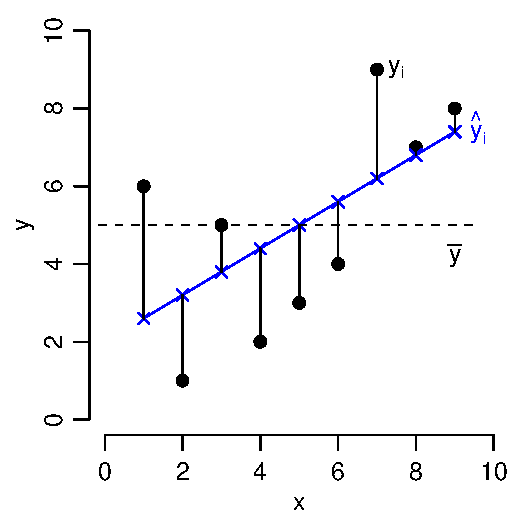
\includegraphics[scale=.7]{figures/obs_pred}
\end{column}
%
\begin{column}{5cm}
{\small
\[
  s_y^2 = s_{\hat y}^2 + s_e^2
\]
\[
  \frac{1}{n} \sum_{i=1}^n (y_i - \bar{y})^2 =
\]
\[
  \frac{1}{n} \sum_{i=1}^n (\hat{y_i} - \bar{y})^2 +
  \frac{1}{n} \sum_{i=1}^n (y_i - \hat{y_i})^2
\]
}
\end{column}
\end{columns}
\vfill
\end{frame}

\begin{frame}{Analysis of Variance (Streuungszerlegung)}
Since the residuals $e_i$ are uncorrelated with $y_i$, we get
\[
  s_y^2 = s_{\hat{y}}^2 + s_e^2
\]
The variance of criterion $y$ can be partitioned into a part that can be
  explained by the regression of $x$ on $y$ and the variance of the
  residuals\\[2ex]

  The corresponding parts of the total variance of $y$ are determined by
  the determination coefficient
\begin{align*}
  s_e^2 &= (1 - r^2) \cdot s_y^2\\
  s_{\hat{y}}^2 &= r^2 \cdot s_y^2
\end{align*}
For the determination coefficient, we therefore get
\[
  r^2 = \frac{s_{\hat{y}}^2}{s_y^2} = 1 - \frac{s_e^2}{s_y^2}
\]
\end{frame}

\subsection{Simple regression analysis}

\begin{frame}{Statistical model}
For the pairs
\[
  (x_1, y_1), \ldots, (x_n, y_n),
\]
we get the stochastical model
\[
  y_i = \alpha + \beta \cdot x_i + \varepsilon_i
\]
($i = 1, \ldots, n$)\\[2ex]

The error variables $\varepsilon_i$ \ldots
\begin{itemize}
\item \ldots are not observable and consist of the uncontrolled or not
  systematically measurable influence of the measurement error or
  additional influencing variables
\item it is therefore reasonable to assume that
\[
  E(\varepsilon_i) = 0, ~\text{for all}~ i = 1, \ldots, n
\]
\end{itemize}
\end{frame}

\begin{frame}{Additional assumptions}
The basic stochastical model
\[
  y_i = \alpha + \beta \cdot x_i + \varepsilon_i ~\text{with}~
  E(\varepsilon_i) = 0, ~\text{for all}~ i = 1, \ldots, n
\]
is extended by additional assumptions

\begin{itemize}
\item The random variables $\varepsilon_i$, $i = 1, \ldots, n$ are assumed
  to be stochastically independent and identically distributed

\item Particularly, all $\varepsilon_i$, $i = 1, \ldots, n$ are assumed
  to have the same variance $Var(\varepsilon_i) = \sigma^2$

\item This means for all $i = 1, \ldots, n$, we get
\[
  E(\varepsilon_i \mid x_i) = 0, ~~
  Var(\varepsilon_i \mid x_i) = \sigma^2
\]
\end{itemize}
\end{frame}


\begin{frame}{Conclusions}
  From the properties of the error variables, we conclude
\[
  E(y_i) = E(\alpha + \beta \cdot x_i + \varepsilon_i) =
  \alpha + \beta \cdot x_i = \bar{y}
\]
and
\[
  Var(y_i) = Var(\alpha + \beta \cdot x_i + \varepsilon_i) = \sigma^2
\]
For a given $x_i$, the stochastical independence of $\varepsilon_i$
  transfers to $y_i$\\[2ex]
\end{frame}

\begin{frame}{}
  \begin{itemize}
    \item 
  \end{itemize}
\end{frame}

\section{}

% \begin{frame}{}
%   \begin{itemize}
%     \item 
%   \end{itemize}
% \end{frame}
% 
{\setbeamercolor{background canvas}{bg=iwmgrau!80!white}

\begin{frame}[fragile]{PBC Example Rizopoulos}
\begin{lstlisting}
# load data
con <- url("https://raw.github.com/drizopoulos/Repeated_Measurements/master/Data.RData")
load(con)
close(con)

# model slide 43
summary(lm(log(serBilir) ~ age + drug, pbc2[pbc2$year == 0, ]))

\end{lstlisting}
\end{frame}

}

% \begin{frame}[fragile]{}
%   \begin{itemize}
%     \item 
% \begin{lstlisting}[style=plain]
% ###
% \end{lstlisting}
%   \end{itemize}
% \end{frame}
% 
% \begin{frame}{}
%   \begin{block}{Exercise}
%     \begin{itemize}
%       \item 
%     \end{itemize}
%   \end{block}
% \end{frame}

\appendix
%\begin{frame}[allowframebreaks]{References}
\begin{frame}{References}
\renewcommand{\bibfont}{\footnotesize}
\bibliographystyle{apacite}
\bibliography{../../../literature/nu}
\vfill
\end{frame}

\end{document}

